\section{Wiring}

A custom microwave processing system was used to generate and detect the measurement pulses.
A simplified diagram of the experimental setup, shown in Fig.\,\ref{Fig:wiring}, serves as the main reference for our discussion.

\subsection{General view}

The microwave probe signals were generated with a custom designed 1\,Gs/s arbitrary waveform generator (AWG) and IQ mixer at room temperature.
The generated signal contains one frequency component for each measurement resonator being probed.
The signal travels through several stages of attenuation at 4\,K and 40\,mK which dissipate thermal and technical noise.
When the measurement pulse arrives at the chip, most of it is reflected from the input capacitor, and a small portion is transmitted into the bandpass filter.
Once inside the filter, each frequency component of the transmitted signal scatters from its corresponding measurement resonator, acquiring a qubit state dependent phase and amplitude shift.
The dispersed signal leaves the chip through the filter tap-off path (red arrow in Fig.\,\ref{Fig:deviceMicrograph}) and enters a series of filters and switches at 40\,mK before it is amplified by a parametric amplifier (paramp).
The signal is then further amplified by a high electron mobility transistor (HEMT) amplifier at 4\,K before it is brought up to room temperature, further amplified, and detected by a custom designed GHz analog to digital converter (ADC).

\begin{figure}
\begin{centering}
\includegraphics[width=\textwidth]{wiringDiagram.pdf} 
\par\end{centering}
\caption{Schematic of the measurement system.}
\label{Fig:wiring}
\end{figure}

\subsection{Noise attenuation and filtering}

The microwave control lines are designed with $50\Omega$ characteristic impedance, as this value is well supported by off-the-shelf commercial microwave hardware, such as cables, connectors, and attenuators.
Therefore, the quantum circuitry is designed under the assumption that the control lines can be modeled as $50\Omega$ \, resistors.
Resistors generate temperature and resistance dependent voltage and current noise \cite{Nyquist:noise1928}, so the qubits and resonators are subjected to noise coming from their control lines at the base temperature of the cryostat, approximately 40\,mK.
We designed the coupling strengths between the control lines and the quantum circuits (qubits and resoantors) such that this 40\,mK noise would not introduce significant decoherence.
However, warmer stages of the cryostat generate thermal noise which exceeds the noise from 40\,mK.
This hotter noise propagates through the lines and could interact with the quantum circuits, violating our design assumption and introducing decoherence.
Therefore, we use filters and attenuators to reduce the noise incoming from hotter stages of the cryostat down to the level of noise generated at 40\,mK.

\subsubsection{Review of thermal noise}

The thermal noise of a resistor $R$, at temperature $T$ follows the Plank distribution \footnote{Note that here spectral densities are written in terms of the root mean square (RMS) of the voltage fluctuations.} \begin{equation}
S^p_V(f, T) = \frac{2R h f}{e^{h f /k_b T} - 1} . \end{equation}
The superscript $p$ in $S^p$ reminds us that this is a ``physicist's'' spectral density defined for both positive and negative frequencies.
For $k_bT \gg h f$ we expand in powers of $hf / k_b T$, finding $S^p_V(f, T) \approx 2R \left( k_b T - h f / 2 \right)$.
Multiplying by a factor of 2 to convert to a single sided ``engineer's'' spectral density, and dropping the small constant $-hf / 2$ we find $S^e_V \approx 4 R k_bT$, which is the usual Johnson noise formula \cite{Johnson:noise1928, Nyquist:noise1928}.

In the Johnson limit, the thermal noise power scales linearly with $T$.
Therefore, in order to reduce noise coming from a high temperature stage at $T_{\text{high}}$ to the level of a lower temperature stage at $T_{\text{low}}$, we attenuate the line by a factor of $T_{\text{high}} / T_{\text{low}}$.

When $k_b T \lesssim h f$, the Johnson formula no longer applies.
In this so-called ``quantum limit'', the thermal noise power scales as $\exp \left[ -hf / k_b T \right]$, which is stronger than the linear scaling in the Johnson limit.
Consequently, in going from $T_{\text{high}}$ to $T_{\text{low}}$, we must attenuate by a factor larger than $T_{\text{high}} / T_{\text{low}}$.
Consider the ratio of thermal noise power from sources at two temperatures for a fixed frequency $f=6\,\text{GHz}$.
Defining a reduced temperature as $x \equiv k_b T / hf$, we write the Planck power distribution as \begin{equation}
S_V(T) \propto \frac{1}{e^{1/x}-1} . \end{equation}
The ratio of the noise power for a source at temperature $\alpha T$ to the noise power from a source at temperature $T$ is
\begin{equation}
\frac{S_V(\alpha T)}{S_V(T)} = \frac{e^{1 / x} - 1}{e^{1 / \alpha x} - 1} . \end{equation}
This function is plotted for the case $T=4\,\text{K}$ ($x=13.8$) and $f=6\,\text{GHz}$ in Fig.\,\ref{Fig:ch:setup:sec:wiring:thermalNoiseRatio}.

\begin{figure}
\begin{centering}
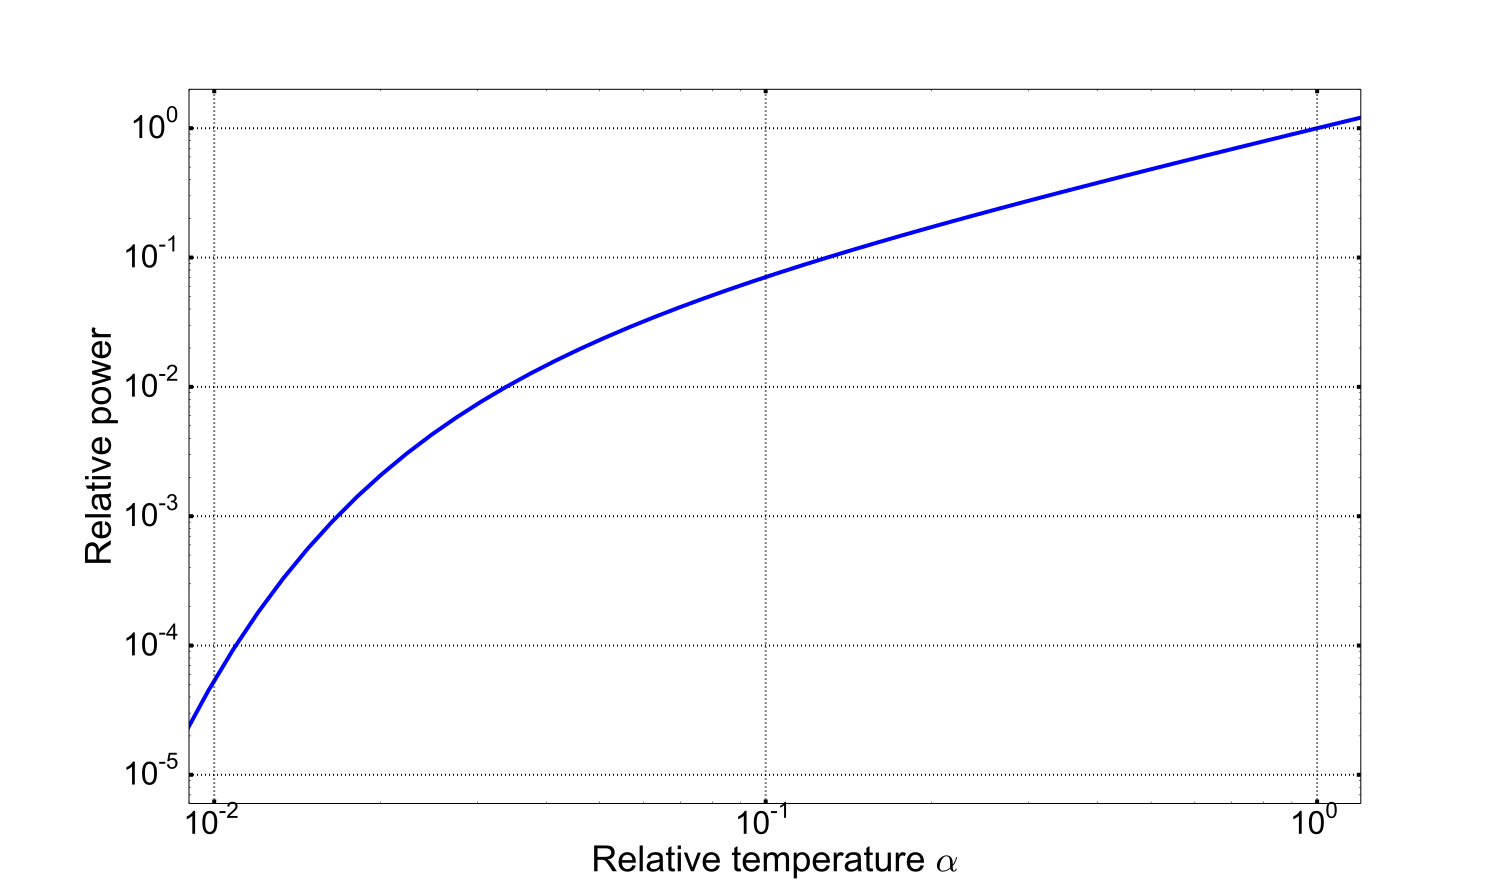
\includegraphics[width=\textwidth]{thermalNoiseRatio.pdf} 
\par\end{centering}
\caption{Ratio of voltage noise spectral density $S_V(\alpha T) / S_V(T)$ for $T=4\,\text{K}$ and $f=6\,\text{GHz}$.}
\label{Fig:ch:setup:sec:wiring:thermalNoiseRatio}
\end{figure}

\subsubsection{Input line}

The qubit, measurement resonator, and filter resonances are all in the 5\,GHz to 7\,GHz range.
For this frequency range, $T_{\text{eff}} \equiv h f / k_b$ is in the range 240\,mK to 335\,mK.
Therefore, the parts of the apparatus at 295\,K (room temperature) and 4\,K are deep in the $k_b T \gg h f$ limit, and we can model their noise properties using the Johnson formula.
Accordingly, we attenuate by a factor of 20\,dB ($\times$100) in between the room temperature and 4\,K stages, as shown in Fig.\,\ref{Fig:wiring}.

The 40\,mK stage is in the quantum limit where $hf \gtrsim k_b T$.
Consequently, the factor of 100 reduction in temperature going from 4\,K to 40\,mK requires more than 20\,dB of attenuation in the line.
In going from 4\,K ($\alpha=1$) to 40\,mK ($\alpha = 10^{-2}$), the thermal noise drops by 5 orders of magnitude, as opposed to 2 orders predicted by the Johnson formula.
We accounted for this by using 30\,dB line attenuation, plus another 20\,dB of isolation from the filter's input capacitor.
In order to remove noise at higher frequencies, we added a 9.6\,GHz low pass reflective filter.
Additionally, an infra-red (IR) filter was used to absorb high frequency radiation propagating down the coaxial transmission line to prevent generation of quasiparticles in the superconductor \cite{Barends:radiation2011}.

\subsubsection{Ground loops}

An inner DC block placed just after the AWG was crucial to the setup.
Without this block, a ground loop introduced kHz frequency signals into the paramp, modulating its gain.
The block broke this ground loop and stabilized the paramp gain.
We also found that care was needed in breaking the grounds between the computer controlling the six port switch and the rest of the apparatus.
In the initial setup, the digital communication line between the computer and the switch control box had the inner and outer conductors broken a different points, almost two meters apart.
This created a large capacitance which allowed transmission of noise from the computer to the control box.
This was fixed by adding a low pass filter where the control box lines entered the cryostat.


\subsection{Output line}

Immediately upon exiting the chip, the measurement signal passes through another reflective low pass filter and IR filter.
No attenuator was used here because loss of measurement photons degrades the quality of the measurement.\footnote{This point is discussed quantitatively in section \ref{sec:measurementInducedDephasing}.} The IR filter introduces $\sim 2\,\text{dB}$ of loss.

The output signal next went through a Radiall R573423600 six port microwave switch.
This allowed us to switch \textit{in-situ} the input to the parametric amplifier.
Switching to calibrated noise sources allowed us to check the noise properties of the paramp.
The signal next passed through a Radiall R572433000 two port switch which allowed us to select between two paramps.
This was done because one of the amplifiers used a new design which was not fully tested and we wanted to have the second amplifier as a fall-back.
The new design turned out to work extremely well and was critical to the success of the experiment.
The signal next entered a circulator which directed it to the paramp where it was amplified and reflected.
The circulator directs the reflected signal toward the second two port switch.
Because the directivity of the circulator is imperfect, some of the reflected amplified signal and noise goes backwards toward the chip.
To eliminate this backward signal, another circulator configured as an isolator was included between the six port switch and the first two port switch.
After leaving the paramp the signal goes through a second two port switch, another circulator configured as an isolator, and then entered a Low Noise Factory HEMT.
The purpose of the paramp was to amplify the measurement signal above the input referred noise of the HEMT, which in this experiment was approximately 2.5\,K.
The unusually low noise of the HEMT was a major advantage as it lowered the requirement on the paramp gain.
After amplification by the HEMT the signal travelled out of the cryostat to room temperature amplifiers which increased the signal level enough to drive an IQ mixer.
The I and Q components generated by the IQ mixer were buffered by custom designed GHz op-amp buffer amplifiers which drove two inputs of a custom Gs/s ADC.
